\section{Netzebenen}

\begin{center}
    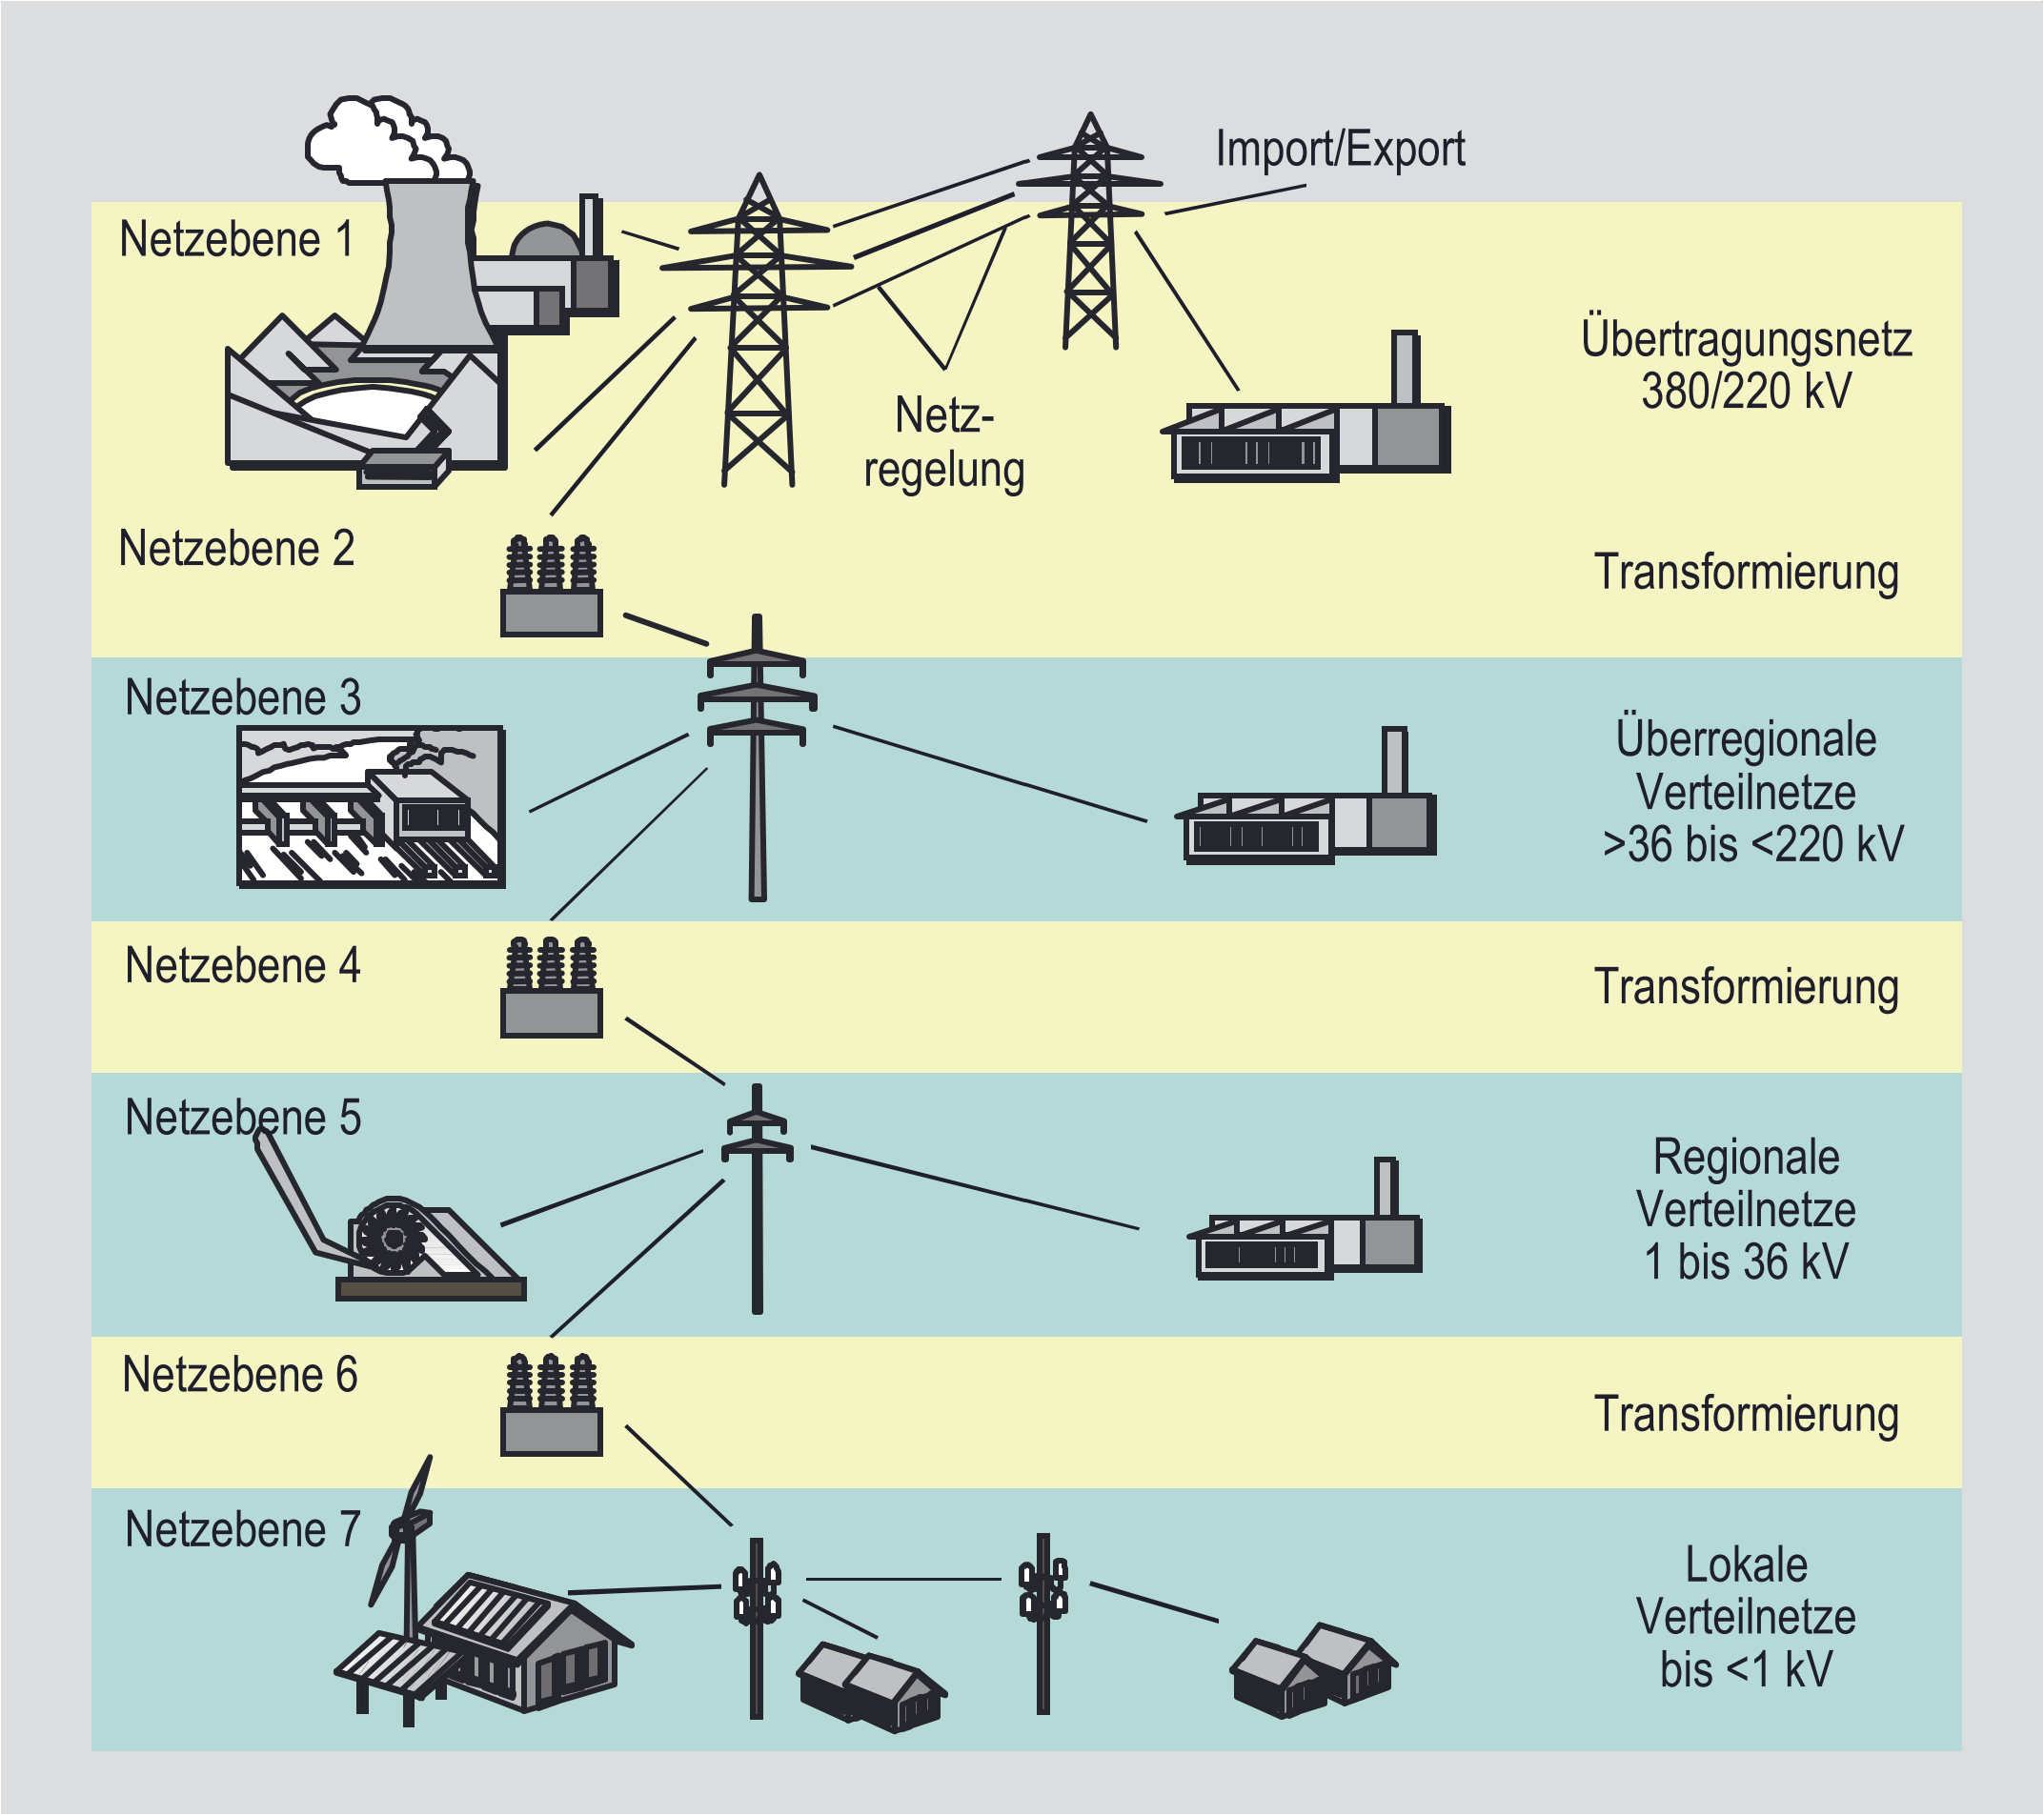
\includegraphics[width=0.95\columnwidth, align=c]{images/Netzebenen_1.png}
\end{center}

\begin{tabular}{>{\bfseries}l l l}
    \toprule
    Spannungsebene & Spannungsbereich & Leistung \\
    \midrule
    Höchstspannung   & 380 kV, 220 kV         & > 300 MVA \\
    Hochspannung     & 150 kV bis 50 kV       & < 100 MVA \\
    Mittelspannung   & 36 kV bis 6 kV         & < 30 MVA \\
    Niederspannung   & 0{,}4 kV               & < 1 MVA \\
    \bottomrule
\end{tabular}

\subsection{NE1: Übertragungsnetz}

\begin{itemize}
    \item 380 kV und 220 kV
    \item Zweck
    \begin{itemize}
        \item Abtransport der großen Kraftwerksleistungen (typ. > 300 MVA)
        \item Versorgung der Verteilnetze
        \item Weiträumiger Energietransport
        \item Internationaler Verbundbetrieb, Energieaustausch
    \end{itemize}
    \item \textbf{Ausdehnung:} national, international
    \item \textbf{Topologie:} (stark) vermaschtes Netz
    \item \textbf{Technologie:} fast ausschließlich Freileitungen
\end{itemize}

\subsubsection{Schweizer Stromübertragungsnetz (Daten 2014)}

\begin{center}
    \includegraphics[width=0.95\columnwidth, align=c]{images/Schweizer_übertragungsnetz.png}
\end{center}

\begin{itemize}
    \item Gesamtlänge Übertragungsnetz Inland: 6700 km
    \begin{itemize}
        \item Länge 380 kV: 1780 km
        \item Länge 220 kV: 4920 km
    \end{itemize}
    
    \item Gesamtzahl Leitungen im Übertragungsnetz: 246
    \begin{itemize}
        \item Leitungen 380 kV: 48
        \item Leitungen 220 kV: 198
    \end{itemize}
    
    \item Anzahl Netzübergänge in das Ausland: 41
\end{itemize}

\subsubsection{Entso-E}

\begin{center}
    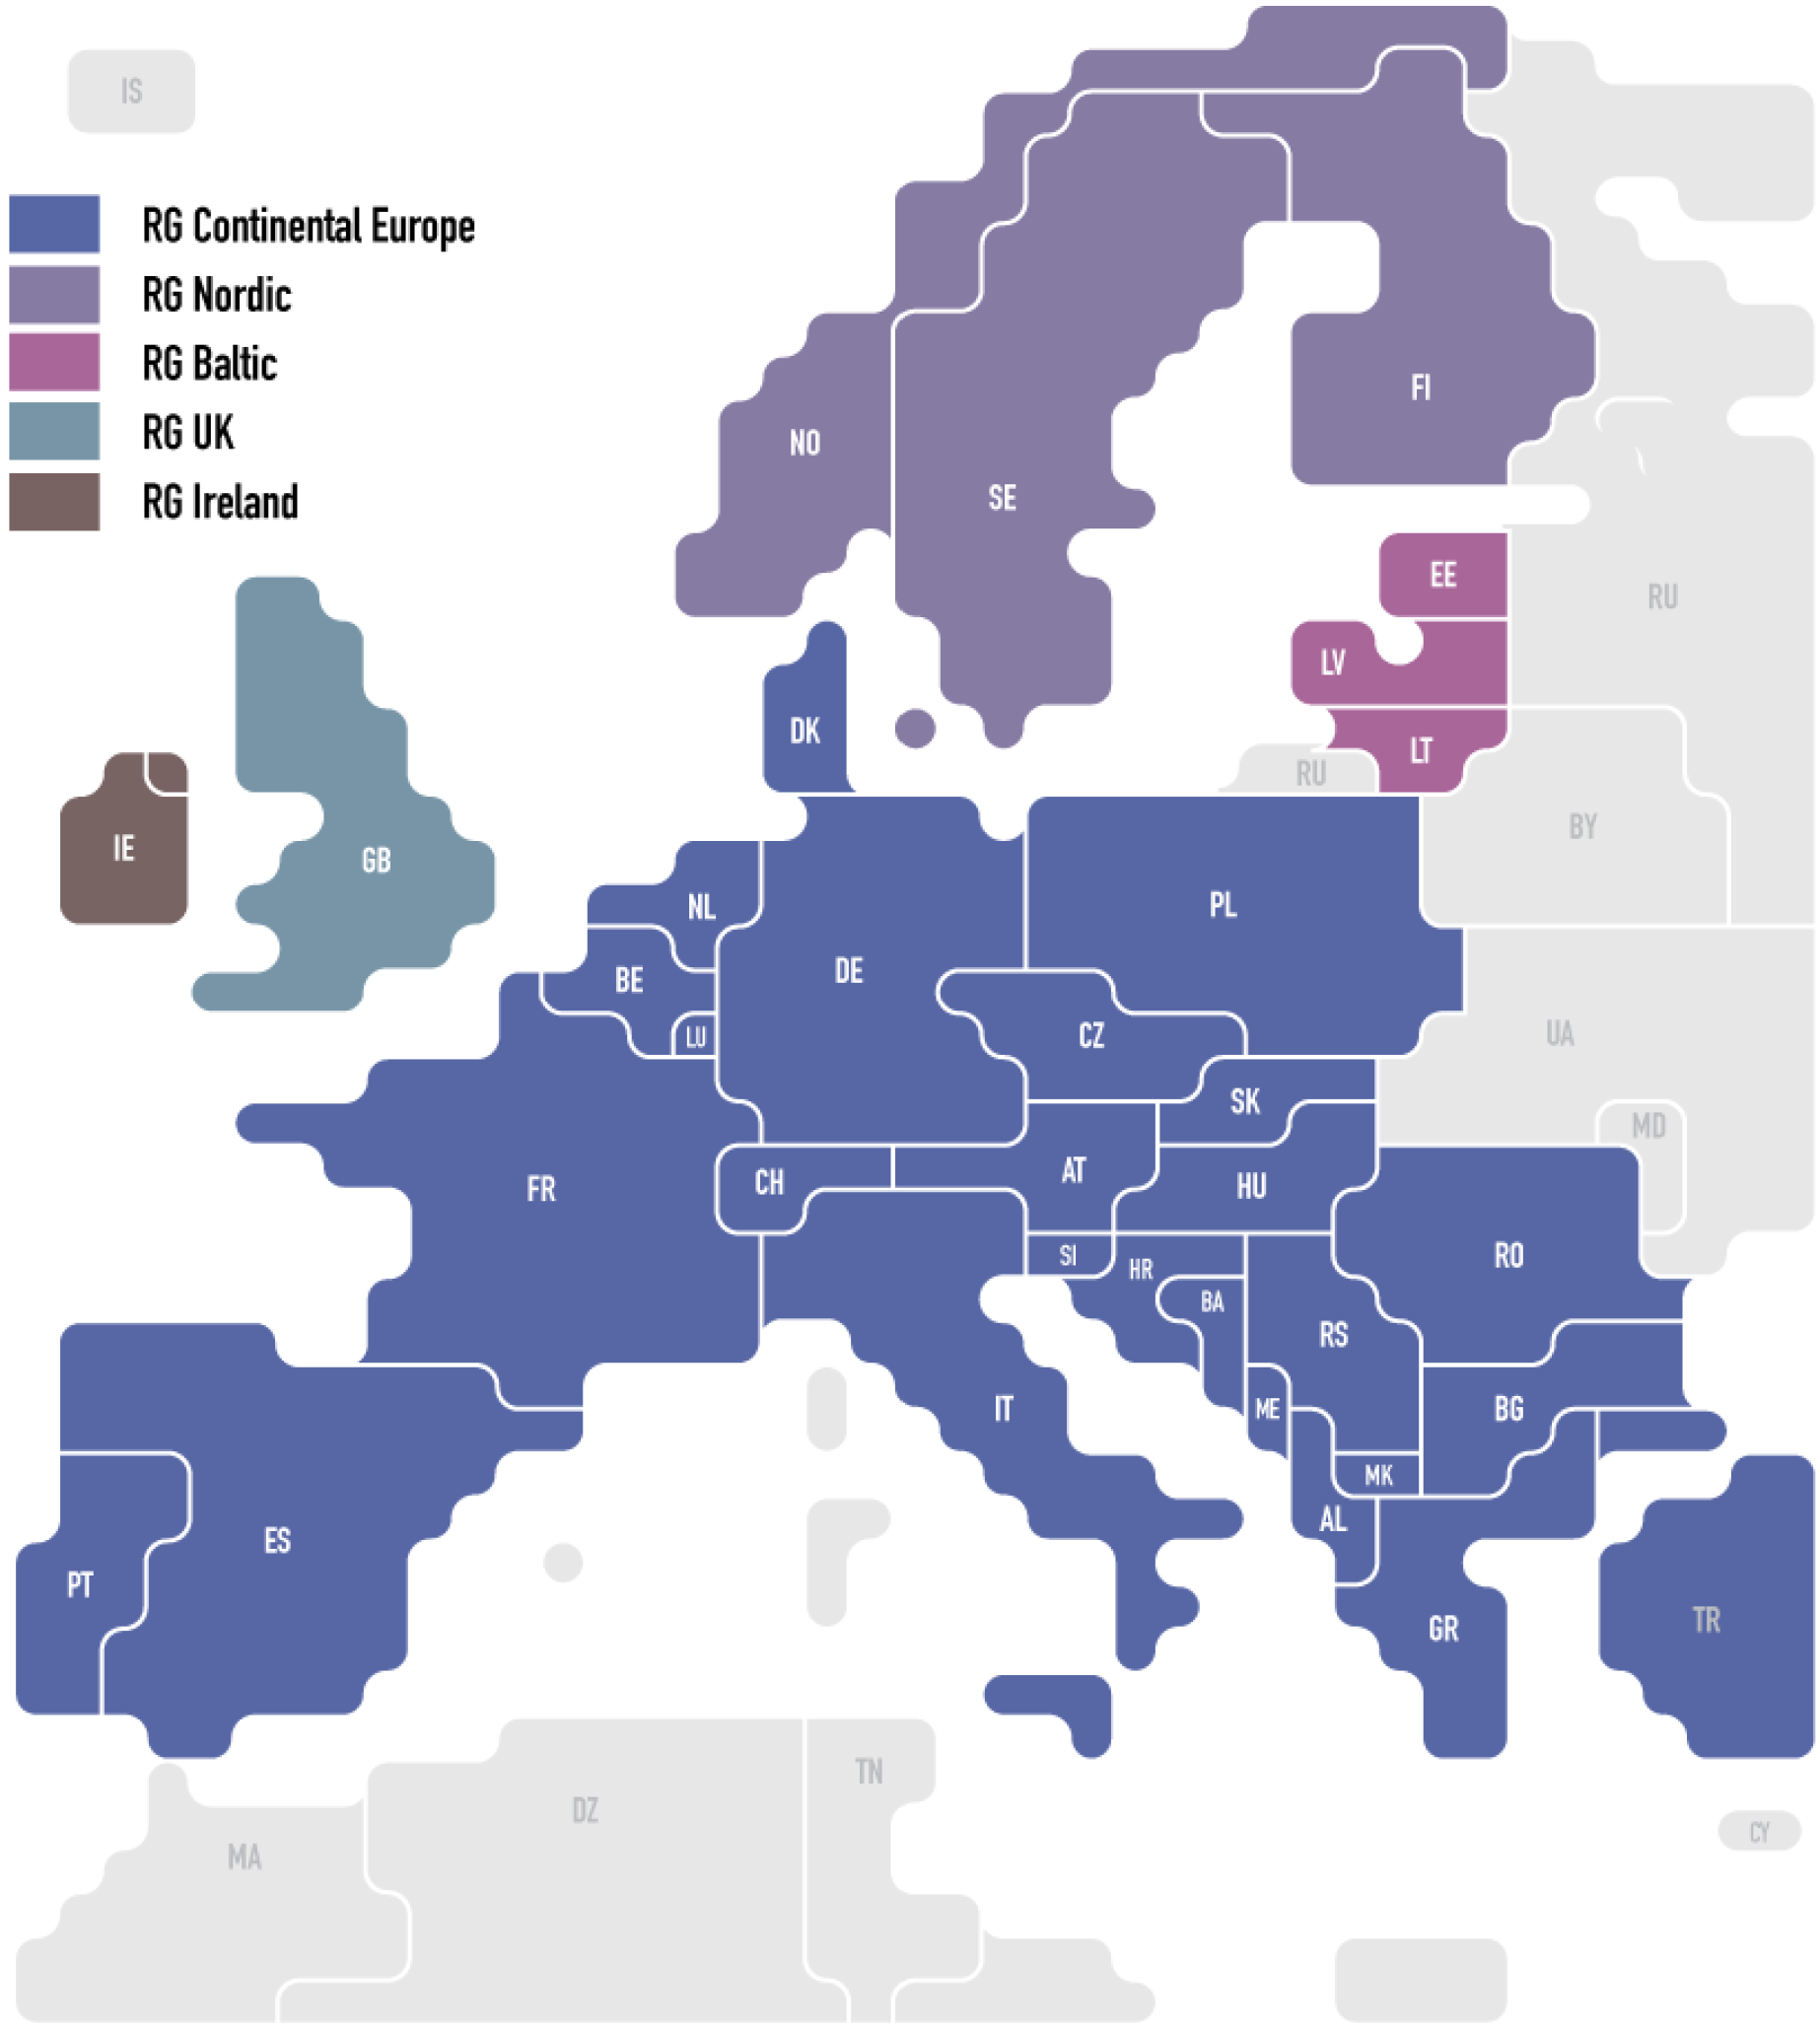
\includegraphics[width=0.95\columnwidth, align=c]{images/Entso_E.png}
\end{center}

\begin{itemize}
    \item koordinierter Systembetrieb
    \item koordinierte Marktlösungen
    \item koordinierte Systementwicklung
\end{itemize}




\subsection{NE3: Überregionales Verteilnetz}

\begin{itemize}
    \item 150 kV, 132 kV, 60 kV
    \item Zweck
    \begin{itemize}
        \item Abtransport mittlerer Kraftwerksleistungen (typ. 100 MVA)
        \item Anschluss großer Industriekunden
        \item Überregionale Verteilung
    \end{itemize}
    \item Ausdehnung: mehrere Kantone
    \item Topologie: (leicht) vermaschtes Netz oder Ringnetz
    \item Technologie: vorwiegend Freileitungen
\end{itemize}

\subsection{NE5: Verteilnetz}


\begin{itemize}
    \item 20 kV, 10 kV
    \item Zweck
    \begin{itemize}
        \item Abtransport kleiner Kraftwerksleistungen (\(< 30\,\text{MVA}\))
        \item Anschluss von Industrie- und Gewerbekunden
        \item Regionale Verteilung
    \end{itemize}
    \item Ausdehnung: Kanton, Tal
    \item Topologie: Ringnetz, Strahlennetz
    \item Technologie: Freileitungen und Kabel
\end{itemize}

\subsection{NE7: Verteilnetz}

\begin{itemize}
    \item 400 V
    \item Zweck
    \begin{itemize}
        \item Abtransport kleinster Einspeisungen (kVA)
        \item Feinverteilung zum Endverbraucher
        \item Anschluss von Haushaltskunden
    \end{itemize}
    \item Ausdehnung: typ. Gemeinde
    \item Topologie: offener Ring, Strahlennetz
    \item Technologie: Freileitungen und Kabel
\end{itemize}





















